\begin{abox}
Practice Set - 1
\end{abox}
\begin{enumerate}
	\item  The electrostatic potential $V(x, y)$ in free space in a region where the charge density $\rho$ is zero is given by $V(x, y)=4 e^{2 x}+f(x)-3 y^{2}$. Given that the $x$-component of the electric field $E_{x}$, and $V$ are zero at the origin, $f(x)$ is
	{\exyear{ NET/JRF(JUNE-2011)}}
	\begin{tasks}(2)
		\task[\textbf{A.}] $3 x^{2}-4 e^{2 x}+8 x$
		\task[\textbf{B.}] $3 x^{2}-4 e^{2 x}+16 x$
		\task[\textbf{C.}] $4 e^{2 x}-8$
		\task[\textbf{D.}] $3 x^{2}-4 e^{2 x}$
	\end{tasks}
	\begin{answer}
		\begin{align*}
		V&=4 e^{2 x}+f(x)-3 y^{2} .\text{ Since }\rho=0 \Rightarrow \nabla^{2} V\\&=0 \Rightarrow 16 e^{2 x}+f^{\prime \prime}(x)-6=0\\
		\text{Since }E_{x}&=0\text{ at origin }\Rightarrow \vec{E}=-\vec{\nabla} V \Rightarrow E_{x}\\&=-\left[8 e^{2 x}+f^{\prime}(x)\right]\\
		E_{x}(0,0)&=-\left[8+f^{\prime}(0)\right]=0 \Rightarrow f^{\prime}(0)=-8\\
		\text{	Since }V(0,0)&=0 \Rightarrow 4+f(0)=0 \Rightarrow f(0)=-4\\
		\text{Solve equation }16 e^{2 x}+f^{\prime \prime}(x)-6&=0 \Rightarrow f^{\prime \prime}(x)=6-16 e^{2 x} \Rightarrow f^{\prime}(x)\\&=6 x-8 e^{2 x}+c_{1},\text{ since}\\
		f^{\prime}(0)&=-8+c_{1}=-8 \Rightarrow c_{1}=0\\
		\text{Again Integrate }f^{\prime}(x)&=6 x-8 e^{2 x} \Rightarrow f(x)=3 x^{2}-4 e^{2 x}+c_{2}\\
		\text{since }f(0)&=-4+c_{2}=-4 \Rightarrow c_{2}\\&=0.\text{ Thus }f(x)=3 x^{2}-4 e^{2 x}
		\end{align*}
		So the correct answer is \textbf{Option (D)}
	\end{answer}
	\item A static, spherically symmetric charge distribution is given by $\rho(r)=\frac{A}{r} e^{-K r}$ where $A$ and $K$ are positive constants. The electrostatic potential corresponding to this charge distribution varies with $r$ as
	{\exyear{NET/JRF(JUNE-2011)}}
	\begin{tasks}(4)
		\task[\textbf{A.}] $r e^{-K r}$
		\task[\textbf{B.}] $\frac{1}{r} e^{-K r}$
		\task[\textbf{C.}] $\frac{1}{r^{2}} e^{-K r}$
		\task[\textbf{D.}] $\frac{1}{r}\left(1-e^{-K r}\right)$
	\end{tasks}
	\begin{answer}
		\begin{align*}
		\text{	since }\nabla^{2} V&=-\rho / \varepsilon_{0}\\
		\nabla^{2} V\text{ must be proportional to }\frac{A}{r} e^{-k r},\text{ where }\nabla^{2} V&=\frac{1}{r^{2}} \frac{\partial}{\partial r}\left(r^{2} \frac{\partial V}{\partial r}\right).
		\end{align*}
		So the correct answer is \textbf{Option (B)}
	\end{answer}
	\item Charges $Q, Q$ and $-2 Q$ are placed on the vertices of an equilateral triangle $A B C$ of sides of length $a$, as shown in the figure. The dipole moment of this configuration of charges, irrespective of the choice of origin, is
	{\exyear{NET/JRF(JUNE-2012)}}
	\begin{figure}[H]
		\centering
		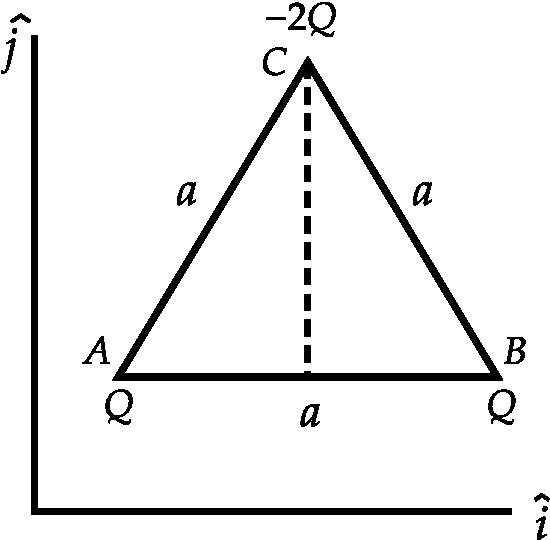
\includegraphics[height=4.5cm,width=4cm]{Electric potential 03}
		\caption{}
		\label{}
	\end{figure}
	\begin{tasks}(4)
		\task[\textbf{A.}] $+2 a Q \hat{i}$
		\task[\textbf{B.}] $+\sqrt{3} a Q \hat{j}$
		\task[\textbf{C.}] $-\sqrt{3} a Q \hat{j}$
		\task[\textbf{D.}] 0
	\end{tasks}
	\begin{answer}
		\begin{align*}
		\intertext{Let coordinates of $A$ is $(l, m)$, then}
		\vec{p}&=q_{i} \vec{r}_{i}^{\prime}=Q[l \hat{i}+m \hat{j}]+Q[(l+a) \hat{i}+m \hat{j}]-2 Q\left[\left(l+\frac{a}{2}\right) \hat{i}+\left(m+\frac{\sqrt{3} a}{2}\right) \hat{j}\right]\\
		\vec{p}&=Q[\hat{i}+m \hat{j}]+Q[(l+a) \hat{i}+m \hat{j}]-Q[(2 l+a) \hat{i}+(2 m+\sqrt{3} a) \hat{j}\rfloor \Rightarrow \vec{p}=-\sqrt{3} a Q \hat{j}
		\end{align*}
		So the correct answer is \textbf{Option (C)}
	\end{answer}
	\item  Four charges (two $+q$ and two $-q$ ) are kept fixed at the four vertices of a square of side $a$ as shown. At the point $P$ which is at a distance $R$ from the centre $(R>>a)$, the potential is proportional to
	{\exyear{NET/JRF(DEC-2012)}}
	\begin{figure}[H]
		\centering
		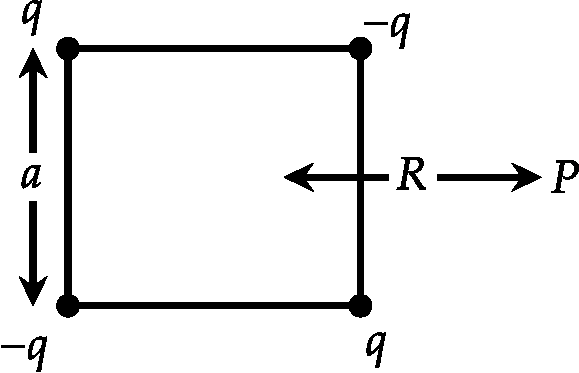
\includegraphics[height=3cm,width=4.2cm]{electric potential 04}
	\end{figure}
	\begin{tasks}(4)
		\task[\textbf{A.}] $1 / R$
		\task[\textbf{B.}] $1 / R^{2}$
		\task[\textbf{C.}] $1 / R^{3}$
		\task[\textbf{D.}] $1 / R^{4}$
	\end{tasks}
	\begin{answer}
		Given configuration is quadrupole.\\
		So the correct answer is \textbf{Option (C)}
	\end{answer}
	\item  A point charges $q$ of mass $m$ is kept at a distance $d$ below a grounded infinite conducting sheet which lies in the $x y$ - plane. For what value of $d$ will the charge remains stationary?
	{\exyear{NET/JRF(DEC-2012)}}
	\begin{tasks}(2)
		\task[\textbf{A.}] $q / 4 \sqrt{m g \pi \varepsilon_{0}}$
		\task[\textbf{B.}] $q / \sqrt{m g \pi \varepsilon_{0}}$
		\task[\textbf{C.}] There is no finite value of $d$
		\task[\textbf{D.}]  $\sqrt{m g \pi \varepsilon_{0}} / q$
	\end{tasks}
	\begin{answer}
		There is attractive force between point charge $q$ and grounded conducting sheet that can be calculate from method of images i.e. $\frac{1}{4 \pi \varepsilon_{0}} \frac{q^{2}}{(2 d)^{2}}=m g \Rightarrow d=\frac{q}{4 \sqrt{m g \pi \varepsilon_{0}}}$\\
		So the correct answer is \textbf{Option (A)}
	\end{answer}
	\item A particle of charge $e$ and mass $m$ is located at the midpoint of the line joining two fixed collinear dipoles with unit charges as shown in the figure. (The particle is constrained to move only along the line joining the dipoles). Assuming that the length of the dipoles is much shorter than their separation, the natural frequency of oscillation of the particle is
	{\exyear{NET/JRF(JUNE-2013)}}
	\begin{figure}[H]
		\centering
		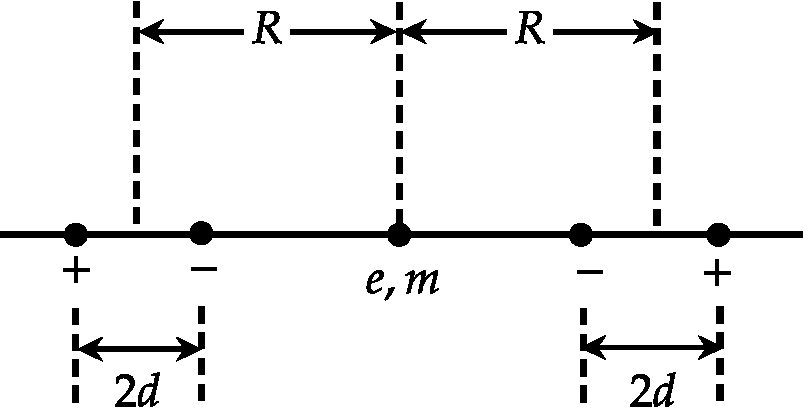
\includegraphics[height=3.5cm,width=7cm]{electric potential 05}
	\end{figure}
	\begin{tasks}(4)
		\task[\textbf{A.}] $\sqrt{\frac{6 e R^{2}}{\pi \varepsilon_{0} m d^{5}}}$
		\task[\textbf{B.}] $\sqrt{\frac{6 e R}{\pi \varepsilon_{0} m d^{4}}}$
		\task[\textbf{C.}]  $\sqrt{\frac{6 e d^{2}}{\pi \varepsilon_{0} m R^{5}}}$
		\task[\textbf{D.}] $\sqrt{\frac{6 e d}{\pi \varepsilon_{0} m R^{4}}}$
	\end{tasks}
	\begin{answer}$\left. \right. $
		\begin{figure}[H]
			\centering
			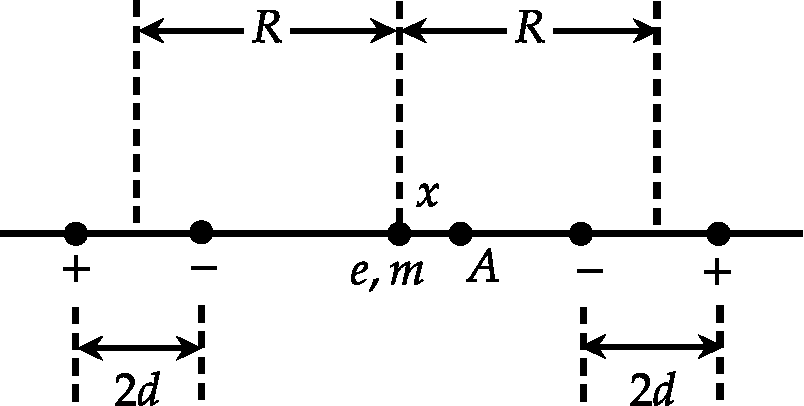
\includegraphics[height=3.5cm,width=7cm]{electric potential 06}
		\end{figure}
		\begin{align*}
		\intertext{Solution: Let us displace the charge particle by small amount $x$ at $A$. Then the resultant electric field at point $A$ is given by}
		E&=\frac{2 p}{4 \pi \varepsilon_{0}}\left[\frac{1}{(R+x)^{3}}-\frac{1}{(R-x)^{3}}\right]=-\frac{6 d}{\pi \varepsilon_{0} R^{4}} x\\
		F&=e E=-\frac{6 e d}{\pi \varepsilon_{0} R^{4}} x .\text{ Then,} \omega=\sqrt{\frac{k}{m}}=\sqrt{\frac{6 e d}{\pi \varepsilon_{0} m R^{4}}}\\
		(\text{where }p&=1 \times 2 d=2 d )
		\end{align*}
		So the correct answer is \textbf{Option (D)}
	\end{answer}
	\item Consider an axially symmetric static charge distribution of the form,
	$$
	\rho=\rho_{0}\left(\frac{r_{0}}{r}\right)^{2} e^{-r / r_{0}} \cos ^{2} \varphi
	$$
	The radial component of the dipole moment due to this charge distribution is
	{\exyear{NET/JRF(JUNE-2013)}}
	\begin{tasks}(4)
		\task[\textbf{A.}] $2 \pi \rho_{0} r_{0}^{4}$
		\task[\textbf{B.}] $\pi \rho_{0} r_{0}^{4}$
		\task[\textbf{C.}] $\rho_{0} r_{0}^{4}$
		\task[\textbf{D.}] $\pi \rho_{0} r_{0}^{4} / 2$
	\end{tasks}
	\begin{answer}
		\begin{align*}
		p&=\int_{V} r^{\prime} \rho\left(r^{\prime}\right) d \tau^{\prime}\\&=\iiint r^{\prime} \times \rho_{0}\left(\frac{r_{0}}{r^{\prime}}\right)^{2} e^{-r^{\prime} / r_{0}} \cos ^{2} \varphi \times r^{\prime 2} \sin \theta d r^{\prime} d \theta d \varphi\\
		p&=\rho_{0} r_{0}^{2} \int_{r^{\prime}=0}^{\infty} r^{\prime} e^{-r^{\prime} / r_{0}} d r^{\pi} \int_{0}^{\pi} \sin \theta d \theta \int_{0}^{2 \pi} \cos ^{2} \varphi d \varphi=2 \pi \rho_{0} r_{0}^{4}
		\end{align*}
		So the correct answer is \textbf{Option (A)}
	\end{answer}
	\item A point charge $q$ is placed symmetrically at a distance $d$ from two perpendicularly placed grounded conducting infinite plates as shown in the figure. The net force on the charge (in units of $1 / 4 \pi \varepsilon_{0}$ ) is
	{\exyear{NET/JRF(DEC-2013)}}
	\begin{figure}[H]
		\centering
		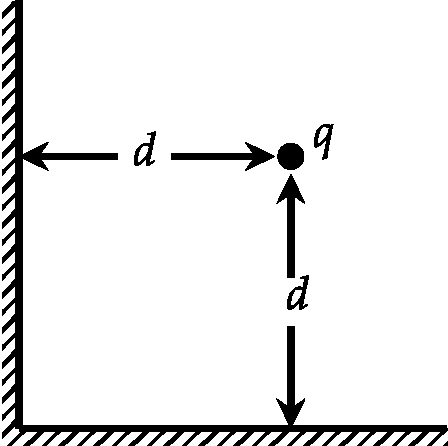
\includegraphics[height=4.5cm,width=5cm]{electric potential 07}
	\end{figure}
	\begin{tasks}(2)
		\task[\textbf{A.}] $\frac{q^{2}}{8 d^{2}}(2 \sqrt{2}-1)$ away from the corner
		\task[\textbf{B.}] $\frac{q^{2}}{8 d^{2}}(2 \sqrt{2}-1)$ towards the corner
		\task[\textbf{C.}] $\frac{q^{2}}{2 \sqrt{2} d^{2}}$ towards the corner
		\task[\textbf{D.}] $\frac{3 q^{2}}{8 d^{2}}$ away from the corner
	\end{tasks}
	\begin{answer}$\left. \right. $
		\begin{figure}[H]
			\centering
			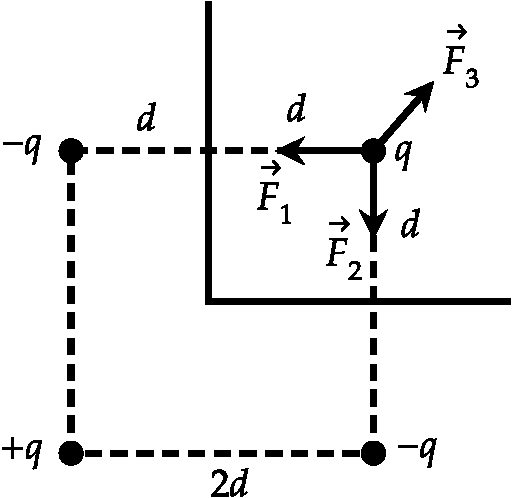
\includegraphics[height=4.5cm,width=5cm]{electric potential 08}
		\end{figure}
		\begin{align*}
		\left|\vec{F}_{1}\right|&=\left|\vec{F}_{2}\right|=k \frac{q^{2}}{4 d^{2}} \text{ and } \left|\vec{F}_{3}\right|=k \frac{q^{2}}{8 d^{2}}\\
		\text{Resultant of }\vec{F}_{1}, \vec{F}_{2}\text{ is }F_{12}&=\sqrt{F_{1}^{2}+F_{2}^{2}}=2 \sqrt{2} k \frac{q^{2}}{8 d^{2}}.\\
		\text{Net force }\vec{F}&=k \frac{q^{2}}{8 d^{2}}(2 \sqrt{2}-1)\text{ (towards the corner)}
		\end{align*}
		So the correct answer is \textbf{Option (B)}
	\end{answer}
	\item If the electrostatic potential $V(r, \theta, \phi)$ in a charge free region has the form $V(r, \theta, \phi)=f(r) \cos \theta$, then the functional form of $f(r)$ (in the following $a$ and $b$ are constants) is:
	{\exyear{NET/JRF(DEC-2013)}}
	\begin{tasks}(4)
		\task[\textbf{A.}] $a r^{2}+\frac{b}{r}$
		\task[\textbf{B.}] $a r+\frac{b}{r^{2}}$
		\task[\textbf{C.}] $a r+\frac{b}{r}$
		\task[\textbf{D.}] $a \ln \left(\frac{r}{b}\right)$
	\end{tasks}
	\begin{answer}
		\begin{align*}
		\nabla^{2} V&=\frac{1}{r^{2}} \frac{\partial}{\partial r}\left(r^{2} \frac{\partial V}{\partial r}\right)+\frac{1}{r^{2} \sin \theta} \frac{\partial}{\partial \theta}\left(\sin \theta \frac{\partial V}{\partial \theta}\right)+\frac{1}{r^{2} \sin ^{2} \theta}\left(\frac{\partial^{2} V}{\partial \phi^{2}}\right)=0\\
		&\Rightarrow \frac{1}{r^{2}} \frac{\partial}{\partial r}\left(r^{2} \frac{\partial f}{\partial r} \cos \theta\right)+\frac{1}{r^{2} \sin \theta} \frac{\partial}{\partial \theta}[\sin \theta f \times(-\sin \theta)]=0\\
		&\Rightarrow \frac{\cos \theta}{r^{2}}\left(r^{2} \frac{\partial^{2} f}{\partial^{2} r}+2 r \frac{\partial f}{\partial r}\right)-\frac{f}{r^{2} \sin \theta}(2 \sin \theta \cos \theta)=0\\
		&\Rightarrow r^{2} \frac{\partial^{2} f}{\partial^{2} r}+2 r \frac{\partial f}{\partial r}-2 f(r)=0\\
		f(r)&=a r+\frac{b}{r^{2}}\text{ satisfy the above equation.}
		\end{align*}
		So the correct answer is \textbf{Option (B)}
	\end{answer}
	\item  Let four point charges $q,-q / 2, q$ and $-q / 2$ be placed at the vertices of a square of side $a$. Let another point charge $-q$ be placed at the centre of the square (see the figure).\\
	\begin{figure}[H]
		\centering
		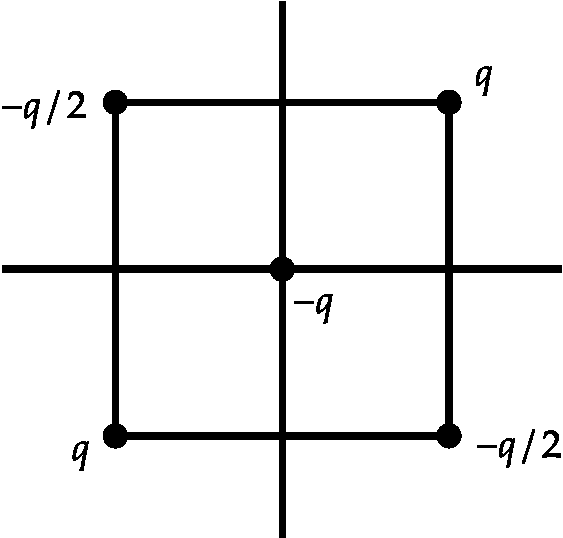
\includegraphics[height=4.5cm,width=5cm]{electric potential 09}
	\end{figure}
	Let $V(r)$ be the electrostatic potential at a point $P$ at a distance $r>>a$ from the centre of the square. Then $V(2 r) / V(r)$ is
	{\exyear{NET/JRF(DEC-2013)}}
	\begin{tasks}(4)
		\task[\textbf{A.}] 1
		\task[\textbf{B.}]  $\frac{1}{2}$
		\task[\textbf{C.}] $\frac{1}{4}$
		\task[\textbf{D.}] $\frac{1}{8}$
	\end{tasks}
	\begin{answer}
		\begin{align*}
		\text{According to multipole expansion }Q_{\text {mono }}&=-\frac{q}{2}+q-\frac{q}{2}+q-q=0
		\intertext{$\vec{p}=q\left(\frac{q}{2} \hat{x}+\frac{q}{2} \hat{y}\right)-\frac{q}{2}\left(-\frac{q}{2} \hat{x}+\frac{q}{2} \hat{y}\right)+0+q\left(-\frac{q}{2} \hat{x}-\frac{q}{2} \hat{y}\right)-\frac{q}{2}\left(\frac{q}{2} \hat{x}-\frac{q}{2} \hat{y}\right)=0$}
		\text{Thus, }V \propto \frac{1}{r^{3}} \Rightarrow \frac{V(2 r)}{V(r)}&=\frac{1}{8}.
		\end{align*}
		So the correct answer is \textbf{Option (D)}
	\end{answer}
	\item If the electrostatic potential in spherical polar coordinates is
	$$
	\varphi(r)=\varphi_{0} e^{-r / r_{0}}
	$$
	where $\varphi_{0}$ and $r_{0}$ are constants, then the charge density at a distance $r=r_{0}$ will be
	{\exyear{NET/JRF(JUNE-2014)}}
	\begin{tasks}(4)
		\task[\textbf{A.}] $\frac{\varepsilon_{0} \varphi_{0}}{e r_{0}^{2}}$
		\task[\textbf{B.}] $\frac{e \varepsilon_{0} \varphi_{0}}{2 r_{0}^{2}}$
		\task[\textbf{C.}] $-\frac{\varepsilon_{0} \varphi_{0}}{e r_{0}^{2}}$
		\task[\textbf{D.}] $-\frac{2 e \varepsilon_{0} \varphi_{0}}{r_{0}^{2}}$
	\end{tasks}
	\begin{answer}
		\begin{align*}
		\because \nabla^{2} \phi&=-\frac{\rho}{\varepsilon_{0}} \Rightarrow \rho=-\varepsilon_{0}\left(\nabla^{2} \phi\right)\\
		\nabla^{2} \phi&=\frac{1}{r^{2}} \frac{\partial}{\partial r}\left(r^{2} \frac{\partial \phi}{\partial r}\right)=\frac{1}{r^{2}} \frac{\partial}{\partial r}\left(r^{2} \times-\frac{\phi_{0}}{r_{0}} e^{-r / r_{0}}\right)\\&=-\frac{1}{r^{2}} \frac{\phi_{0}}{r_{0}} \frac{\partial}{\partial r}\left(r^{2} \times e^{-r / r_{0}}\right)\\
		\Rightarrow \nabla^{2} \phi&=-\frac{1}{r^{2}} \frac{\phi_{0}}{r_{0}}\left[r^{2} \times-\frac{1}{r_{0}} e^{-r / r_{0}}+2 r e^{-r / r_{0}}\right]\\&=-\frac{\phi_{0}}{r_{0}}\left[-\frac{1}{r_{0}} e^{-r / r_{0}}+\frac{2}{r} e^{-r / r_{0}}\right]\\
		\text{At a distance }r&=r_{0}, \quad \nabla^{2} \phi=-\frac{\phi_{0}}{r_{0}}\left[\frac{-1}{r_{0}} e^{-1}+\frac{2}{r_{0}} e^{-1}\right]\\&=-\frac{\phi_{0}}{r_{0}^{2} e} \Rightarrow \rho=-\varepsilon_{0}\left(-\frac{\phi_{0}}{r_{0}^{2} e}\right)=\frac{\phi_{0} \varepsilon_{0}}{r_{0}^{2} e}
		\end{align*}
		So the correct answer is \textbf{Option (A)}
	\end{answer}
	\item A charge $(-e)$ is placed in vacuum at the point $(d, 0,0)$, where $d>0 .$ The region $x \leq 0$ is filled uniformly with a metal. The electric field at the point $\left(\frac{d}{2}, 0,0\right)$ is
	{\exyear{NET/JRF(JUNE-2014)}}
	\begin{tasks}(2)
		\task[\textbf{A.}]  $-\frac{10 e}{9 \pi \varepsilon_{0} d^{2}}(1,0,0)$
		\task[\textbf{B.}]  $\frac{10 e}{9 \pi \varepsilon_{0} d^{2}}(1,0,0)$
		\task[\textbf{C.}] $\frac{e}{\pi \varepsilon_{0} d^{2}}(1,0,0)$
		\task[\textbf{D.}] $-\frac{e}{\pi \varepsilon_{0} d^{2}}(1,0,0)$
	\end{tasks}
	\begin{answer}$\left. \right. $
		\begin{figure}[H]
			\centering
			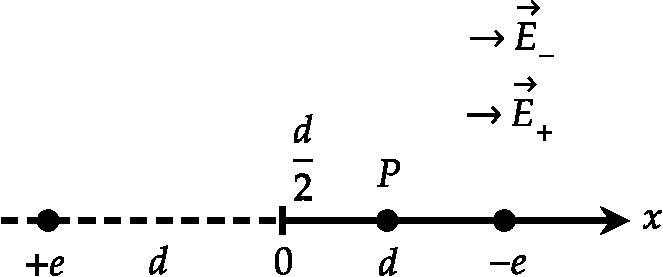
\includegraphics[height=3cm,width=6.5cm]{electric potential 10}
		\end{figure}
		\begin{align*}
		E_{+}&=\frac{1}{4 \pi \varepsilon_{0}} \frac{e}{(3 d / 2)^{2}}=\frac{1}{4 \pi \varepsilon_{0}} \frac{4 e}{9 d^{2}}\text{ and }E_{-}\\&=\frac{1}{4 \pi \varepsilon_{0}} \frac{e}{(d / 2)^{2}}=\frac{1}{4 \pi \varepsilon_{0}} \frac{4 e}{d^{2}}
		\intertext{Thus resultant electric field at point $P$ is}
		E&=E_{+}+E_{-}=\frac{1}{4 \pi \varepsilon_{0}} \frac{4 e}{9 d^{2}}+\frac{1}{4 \pi \varepsilon_{0}} \frac{4 e}{d^{2}}\\&=\frac{1}{4 \pi \varepsilon_{0}} \frac{40 e}{9 d^{2}}=\frac{1}{9 \pi \varepsilon_{0}} \frac{10 e}{d^{2}} \Rightarrow \vec{E}=\frac{1}{9 \pi \varepsilon_{0}} \frac{10 e}{d^{2}} \hat{x}
		\end{align*}
		So the correct answer is \textbf{Option (B)}
	\end{answer}
	\item A charged particle is at a distance $d$ from an infinite conducting plane maintained at zero potential. When released from rest, the particle reaches a speed $u$ at a distance $d / 2$ from the plane. At what distance from the plane will the particle reach the speed $2 u ?$
	{\exyear{NET/JRF(JUNE-2014)}}
	\begin{tasks}(4)
		\task[\textbf{A.}] $d / 6$
		\task[\textbf{B.}] $d / 3$
		\task[\textbf{C.}] $d / 4$
		\task[\textbf{D.}] $d / 5$
	\end{tasks}
	\begin{answer}$\left. \right. $
		\begin{figure}[H]
			\centering
			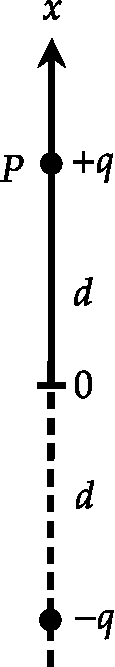
\includegraphics[height=5cm,width=1cm]{electric potential 11}
		\end{figure}
		\begin{align*}
		F&=m a=m \frac{d^{2} x}{d t^{2}}=-\frac{1}{4 \pi \varepsilon_{0}} \frac{q^{2}}{4 d^{2}} \Rightarrow \frac{d^{2} x}{d t^{2}}\\&=-\frac{A}{x^{2}}\text{ where }A=\frac{q^{2}}{16 \pi m \varepsilon_{0}}\\
		\Rightarrow \frac{d v}{d t}&=-\frac{A}{x^{2}} \Rightarrow v \frac{d v}{d t}\\&=-\frac{A}{x^{2}} \frac{d x}{d t} \Rightarrow \frac{1}{2} \frac{d}{d t}\left(v^{2}\right)=\frac{d}{d t}\left(\frac{A}{x}\right)\\
		\Rightarrow \frac{v^{2}}{2}&=\frac{A}{x}+C\text{ at }\Rightarrow x=d, v\\&=0 \Rightarrow C=-\frac{A}{d} \Rightarrow v=\sqrt{2 A} \sqrt{\left(\frac{1}{x}-\frac{1}{d}\right)}\\
		\text{Thus }u&=\sqrt{2 A} \sqrt{\left(\frac{1}{d / 2}-\frac{1}{d}\right)}=\sqrt{\frac{2 A}{d}}\text{ then }2 u\\&=\sqrt{2 A} \sqrt{\left(\frac{1}{x}-\frac{1}{d}\right)} \Rightarrow x=\frac{d}{5}
		\end{align*}
		So the correct answer is \textbf{Option (D)}
	\end{answer}
	\item  The electrostatic lines of force due to a system of four point charges is sketched here. At large distance $r$, the leading asymptotic behaviour of the electrostatic potential is proportional to
	{\exyear{NET/JRF(DEC-2014)}}
	\begin{figure}[H]
		\centering
		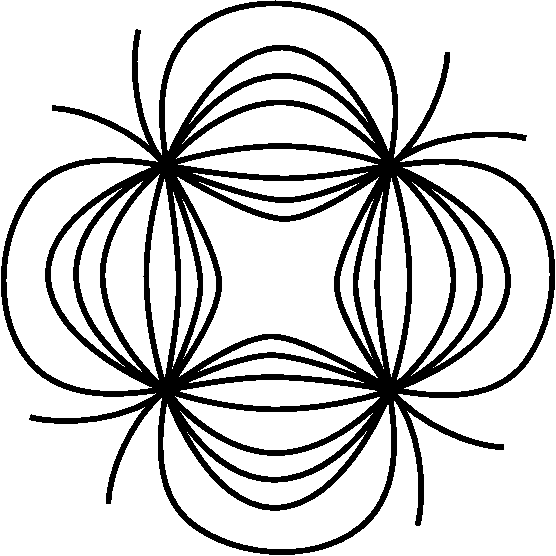
\includegraphics[height=4.5cm,width=4cm]{electric potential 12}
	\end{figure}
	\begin{tasks}(4)
		\task[\textbf{A.}] $r$
		\task[\textbf{B.}] $r^{-1}$
		\task[\textbf{C.}] $r^{-2}$
		\task[\textbf{D.}] $r^{-3}$
	\end{tasks}
	\begin{answer}
		The given electrostatic line of force is due to a quadrupole. So $V \propto \frac{1}{r^{3}}$.\\
		So the correct answer is \textbf{Option (D)}
	\end{answer}
	\item A hollow metallic sphere of radius $a$, which is kept at a potential $V_{0}$ has a charge $Q$ at its centre. The potential at a point outside the sphere, at a distance $r$ from the centre, is
	{\exyear{NET/JRF(DEC-2015)}}
	\begin{tasks}(4)
		\task[\textbf{A.}] $V_{0}$
		\task[\textbf{B.}] $\frac{Q}{4 \pi \in_{0} r}+\frac{V_{0} a}{r}$
		\task[\textbf{C.}] $\frac{Q}{4 \pi \in_{0} r}+\frac{V_{0} a^{2}}{r^{2}}$
		\task[\textbf{D.}] $\frac{V_{0} a}{r}$
	\end{tasks}
	\begin{answer}
		\begin{align*}
		\text{Let charge on conductor is $Q$, then }V_{0}&=\frac{Q}{4 \pi \in_{0} a}\\
		\text{Now }\quad V&=\frac{Q}{4 \pi \in_{0} r} \Rightarrow V=\frac{V_{0} a}{r}
		\end{align*}
		So the correct answer is \textbf{Option (D)}
	\end{answer}
	\item Two uniformly charged insulating solid spheres $A$ and $B$, both of radius $a$, carry total charges $+Q$ and $-Q$, respectively. The spheres are placed touching each other as shown in the figure.\\
	\begin{figure}[H]
		\centering
		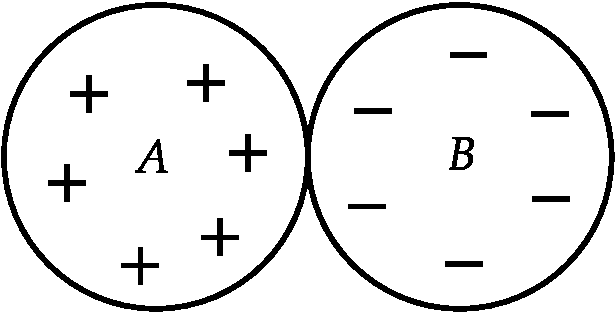
\includegraphics[height=2.5cm,width=4.7cm]{diagram-20211011(50)-crop}
	\end{figure}
	If the potential at the centre of the sphere $A$ is $V_{A}$ and that at the centre of $B$ is $V_{B}$ then the difference $V_{A}-V_{B}$ is
	{\exyear{NET/JRF(DEC-2016)}}
	\begin{tasks}(4)
		\task[\textbf{A.}] $\frac{Q}{4 \pi \varepsilon_{0} a}$
		\task[\textbf{B.}] $\frac{-Q}{2 \pi \varepsilon_{0} a}$
		\task[\textbf{C.}] $\frac{Q}{2 \pi \varepsilon_{0} a}$
		\task[\textbf{D.}] $\frac{-Q}{4 \pi \varepsilon_{0} a}$
	\end{tasks}
	\begin{answer}
		\begin{align*}
		V_{A}&=\frac{3 Q}{8 \pi \in_{0} a}-\frac{Q}{4 \pi \in_{0}(2 a)}=\frac{Q}{4 \pi \in_{0} a}\\
		V_{B}&=\frac{-3 Q}{8 \pi \in_{0} a}+\frac{Q}{4 \pi \in_{0}(2 a)}=\frac{-Q}{4 \pi \in_{0} a}\\
		V_{A}-V_{B}&=\frac{Q}{2 \pi \in_{0} a}
		\end{align*}
		So the correct answer is \textbf{Option (C)}
	\end{answer}
	\item Two long hollow co-axial conducting cylinders of radii $R_{1}$ and $R_{2}\left(R_{1}<R_{2}\right)$ are placed in vacuum as shown in the figure below.\\
	\begin{figure}[H]
		\centering
		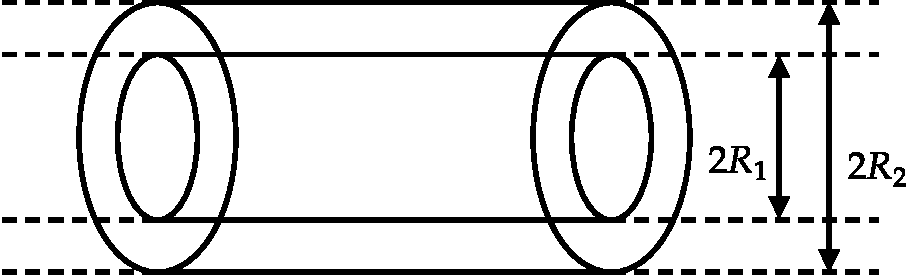
\includegraphics[height=2.5cm,width=7.5cm]{electric potential 13}
	\end{figure}
	The inner cylinder carries a charge $+\lambda$ per unit length and the outer cylinder carries a charge $-\lambda$ per unit length. The electrostatic energy per unit length of this system is
	{\exyear{NET/JRF(JUNE-2017)}}
	\begin{tasks}(2)
		\task[\textbf{A.}] $\frac{\lambda^{2}}{\pi \in_{0}} \ln \left(R_{2} / R_{1}\right)$
		\task[\textbf{B.}] $\frac{\lambda^{2}}{4 \pi \epsilon_{0}}\left(R_{2}^{2} / R_{1}^{2}\right)$
		\task[\textbf{C.}] $\frac{\lambda^{2}}{4 \pi \epsilon_{0}} \ln \left(R_{2} / R_{1}\right)$
		\task[\textbf{D.}] $\frac{\lambda^{2}}{2 \pi \epsilon_{0}} \ln \left(R_{2} / R_{1}\right)$
	\end{tasks}
	\begin{answer}
		\begin{align*}
		r<R_{1}, \vec{E}_{1}&=0 ; R_{1}<r<R_{2}, \vec{E}_{2}=\frac{\lambda}{2 \pi \in_{0} r} \hat{r}\\
		r>R_{z}, \quad \vec{E}_{3}&=0\\
		W&=\frac{\epsilon_{0}}{2} \int_{\text {all spce }}{E^{2} d z}=\frac{\epsilon_{0}}{2} \int_{R_{1}}^{R z} \frac{\lambda^{2}}{4 \pi^{2} \in_{0}^{2} r^{2}} \times 2 \pi r l d r\\
		\frac{W}{l}&=\frac{\epsilon_{0}}{2} \times \frac{\lambda^{2}}{2 \pi \epsilon_{0}^{2}} \int_{R_{1}}^{R_{2}} \frac{1}{r} d r=\frac{\lambda^{2}}{4 \pi \in_{0}} \ln \left(\frac{R_{2}}{R_{1}}\right)
		\end{align*}
		So the correct answer is \textbf{Option (C)}
	\end{answer}
	\item Two point charges $+3 Q$ and $-Q$ are placed at $(0,0, d)$ and $(0,0,2 d)$ respectively, above an infinite grounded conducting sheet kept in the $x y$ - plane. At a point $(0,0, z)$, where $z>>d$, the electrostatic potential of this charge configuration would approximately be
	{\exyear{NET/JRF(DEC-2017)}}
	\begin{tasks}(4)
		\task[\textbf{A.}] $\frac{1}{4 \pi \varepsilon_{0}} \frac{d^{2}}{z^{3}} Q$
		\task[\textbf{B.}] $\frac{1}{4 \pi \varepsilon_{0}} \frac{2 d}{z^{2}} Q$
		\task[\textbf{C.}] $\frac{1}{4 \pi \varepsilon_{0}} \frac{3 d}{z^{2}} Q$
		\task[\textbf{D.}] $-\frac{1}{4 \pi \varepsilon_{0}} \frac{d^{2}}{z^{3}} Q$
	\end{tasks}
	\begin{answer}$\left. \right. $
		\begin{figure}[H]
			\centering
			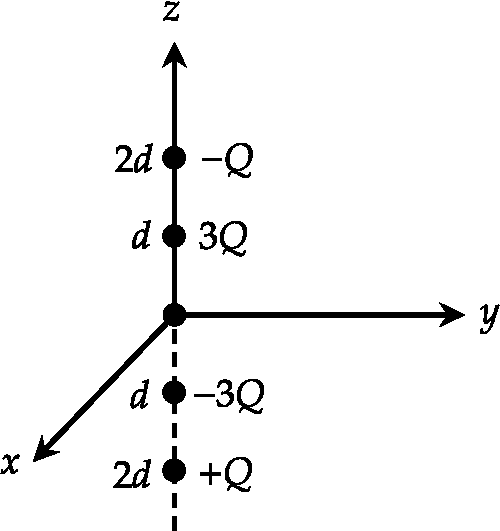
\includegraphics[height=5cm,width=4.5cm]{electric potential 14}
		\end{figure}
		\begin{align*}
		\text{Monopole moment }Q_{\text {mono }}&=-Q+3 Q-3 Q+Q=0\\
		\text{Dipole moment }\vec{p}&=+3 Q \times(d \hat{z})+(-Q) \times(2 d \hat{z})+(-3 Q) \times(-d \hat{z})+Q \times(-2 d \hat{z})\\
		\vec{p}&=2 Q d \hat{z}\\
		V_{d i p}&=\frac{1}{4 \pi \in_{0}} \frac{\vec{p} \cdot \hat{r}}{r^{2}} \approx \frac{1}{4 \pi \in_{0}} \frac{2 Q d}{z^{2}}
		\end{align*}
		So the correct answer is \textbf{Option (B)}
	\end{answer}
	\item  Two point charges $+2 Q$ and $-Q$ are kept at point with Cartesian coordinates $(1,0,0)$, respectively, in front of an infinite grounded conducting plate at $x=0$. The potential at $(x, 0,0)$ for $x \gg 1$ depends on $x$ as
	{\exyear{NET/JRF(JUNE-2018)}}
	\begin{tasks}(4)
		\task[\textbf{A.}] $x^{-3}$
		\task[\textbf{B.}]  $x^{-5}$
		\task[\textbf{C.}] $x^{-2}$
		\task[\textbf{D.}] $x^{-4}$
	\end{tasks}
	\begin{answer}$\left. \right. $
		\begin{figure}[H]
			\centering
			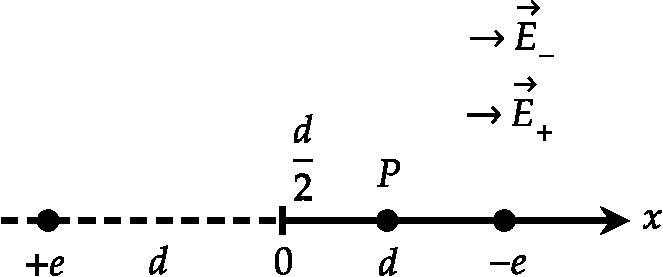
\includegraphics[height=2.5cm,width=5.5cm]{electric potential 16}
		\end{figure}
		\begin{align*}
		\text{Monopole moment }&2 Q-Q-2 Q+Q=0\\
		\text{Dipole moment }\vec{p}&=-Q(2 \hat{x})+2 Q(\hat{x})-2 Q(-\hat{x})+Q(-2 \hat{x}) \Rightarrow \vec{p}=0\\
		\text{Thus }V &\propto \frac{1}{x^{3}}
		\end{align*}
		So the correct answer is \textbf{Option (A)}
	\end{answer}
	\item An electric dipole of dipole moment $\vec{P}=q b \hat{i}$ is placed at origin in the vicinity of two charges $+q$ and $-q$ at $(L, b)$ and $(L,-b)$, respectively, as shown in the figure. The electrostatic potential at the point $\left(\frac{L}{2}, 0\right)$ is
	{\exyear{NET/JRF(DEC-2018)}}
	\begin{figure}[H]
		\centering
		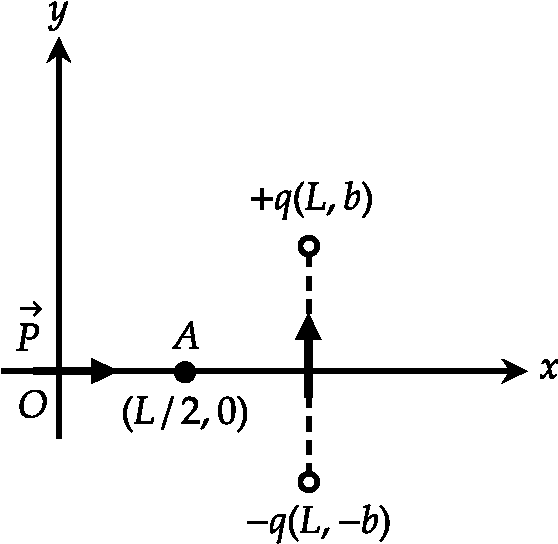
\includegraphics[height=5cm,width=5cm]{electric potential 15}
	\end{figure}
	\begin{tasks}(4)
		\task[\textbf{A.}] $\frac{q b}{\pi \varepsilon_{0}}\left(\frac{1}{L^{2}}+\frac{2}{L^{2}+4 b^{2}}\right)$
		\task[\textbf{B.}] $\frac{4 q b L}{\pi \varepsilon_{0}\left[L^{2}+4 b^{2}\right]^{3 / 2}}$
		\task[\textbf{C.}] $\frac{q b}{\pi \varepsilon_{0} L^{2}}$
		\task[\textbf{D.}] $\frac{3 q b}{\pi \varepsilon_{0} L^{2}}$
	\end{tasks}
	\begin{answer}
		\begin{align*}
		\text{Potential due to dipole }V_{1}&=\frac{1}{4 \pi \varepsilon_{0}} \frac{p \cos 0^{0}}{(L / 2)^{2}}=\frac{1}{\pi \varepsilon_{0}} \frac{p}{L^{2}}\\
		\text{Potential due to $+q$ charge }V_{2}&=\frac{1}{4 \pi \varepsilon_{0}} \frac{q}{\sqrt{L^{2} / 4+b^{2}}}\\
		\text{Potential due to $-q$ charge }V_{3}&=-\frac{1}{4 \pi \varepsilon_{0}} \frac{q}{\sqrt{L^{2} / 4+b^{2}}}\\
		\text{	Resultant }V&=V_{1}+V_{2}+V_{3}\\&=\frac{1}{\pi \varepsilon_{0}} \frac{p}{L^{2}} \Rightarrow V=\frac{1}{\pi \varepsilon_{0}} \frac{q b}{L^{2}}
		\end{align*}
		So the correct answer is \textbf{Option (C)}
	\end{answer}
	
	
	
\end{enumerate}
 \colorlet{ocre1}{ocre!70!}
\colorlet{ocrel}{ocre!30!}
\setlength\arrayrulewidth{1pt}
\begin{table}[H]
	\centering
	\arrayrulecolor{ocre}
	\begin{tabular}{|p{1.5cm}|p{1.5cm}||p{1.5cm}|p{1.5cm}|}
		\hline
		\multicolumn{4}{|c|}{\textbf{Answer key}}\\\hline\hline
		\rowcolor{ocrel}Q.No.&Answer&Q.No.&Answer\\\hline
		1&\textbf{D} &2&\textbf{B}\\\hline 
		3&\textbf{C} &4&\textbf{C} \\\hline
		5&\textbf{A} &6&\textbf{D} \\\hline
		7&\textbf{A}&8&\textbf{B}\\\hline
		9&\textbf{B}&10&\textbf{D}\\\hline
		11&\textbf{A} &12&\textbf{B}\\\hline
		13&\textbf{D}&14&\textbf{D}\\\hline
		15&\textbf{D}&16&\textbf{C}\\\hline
		17&\textbf{C} &18&\textbf{B}\\\hline 
		19&\textbf{A} &20&\textbf{C} \\\hline
	\end{tabular}
\end{table}
\begin{abox}
	Practice Set - 2
\end{abox}
\begin{enumerate}
	\item 	 An insulating sphere of radius $a$ carries a charge density
	$$
	\rho(\vec{r})=\rho_{0}\left(a^{2}-r^{2}\right) \cos \theta ; r<a
	$$
	The leading order term for the electric field at a distance $d$, far away from the charge distribution, is proportional to
	{\exyear{GATE 2010}}

\begin{tasks}(4)
\task[\textbf{A.}] $d^{-1}$
\task[\textbf{B.}] $d^{-2}$
\task[\textbf{C.}] $d^{-3}$
\task[\textbf{D.}] $d^{-4}$
\end{tasks}
\begin{answer}
	\begin{align*}
	V(r)&=\left[\frac{1}{r} \int_{V} \rho d \tau+\frac{1}{r^{2}} \int \rho \cos \theta d \tau+\cdots\right]\\
	\mathrm{I}^{\mathrm{st}}\text{ term, }\int \rho d \tau&=\int_{0}^{a} \int_{0}^{\pi} \int_{0}^{2 \pi} \rho_{0}\left(a^{2}-r^{2}\right) \cos \theta \times r^{2} \sin \theta d r d \theta d \phi=0\\
	\mathrm{II}^{\mathrm{nd}}\text{ term, }\int \rho \cos \theta d \tau&=\int_{0}^{a} \int_{0}^{\pi} \int_{0}^{2 \pi} \rho_{0}\left(a^{2}-r^{2}\right) \cos ^{2} \theta \times r^{2} \sin \theta d r d \theta d \phi \neq 0\\
	&\Rightarrow \mathrm{V} \alpha \frac{1}{\mathrm{r}^{2}} \Rightarrow E \alpha \frac{1}{\mathrm{r}^{3}}
	\end{align*}
	So the correct answer is \textbf{Option (C)}
\end{answer}
\item Two charges $q$ and $2 q$ are placed along the $x$ -axis in front of a grounded, infinite conducting plane, as shown in the figure. They are located respectively at a distance of $0.5 \mathrm{~m}$ and $1.5 \mathrm{~m}$ from the plane. The force acting on the charge $q$ is
{\exyear{GATE 2011}}

\begin{figure}[H]
\centering
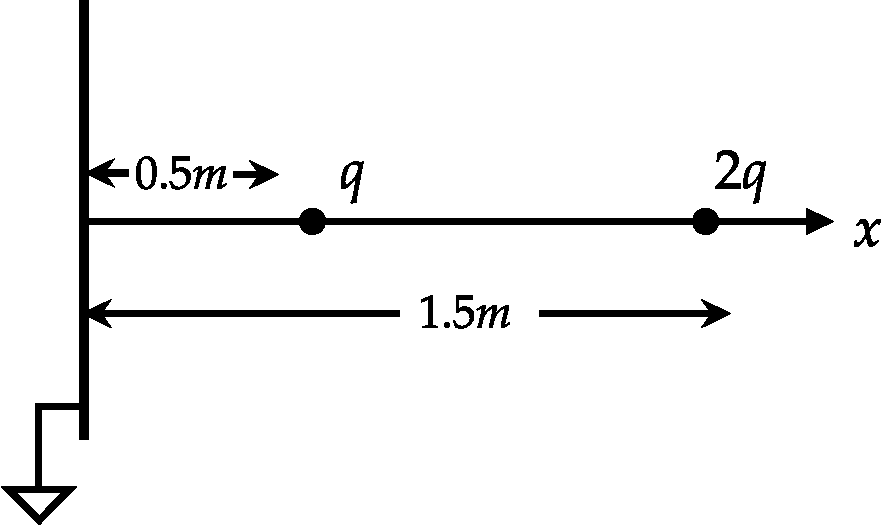
\includegraphics[height=4cm,width=7.5cm]{diagram-20210817(15)-crop}
\end{figure}
\begin{tasks}(4)
\task[\textbf{A.}] $\frac{1}{4 \pi \varepsilon_{0}} \frac{7 q^{2}}{2}$
\task[\textbf{B.}] $\frac{1}{4 \pi \varepsilon_{0}} 2 q^{2}$
\task[\textbf{C.}] $\frac{1}{4 \pi \varepsilon_{0}} q^{2}$
\task[\textbf{D.}] $\frac{1}{4 \pi \varepsilon_{0}} \frac{q^{2}}{2}$
\end{tasks}
\begin{answer}
Using method of Images we can draw equivalent figure as shown below:\\
\begin{figure}[H]
	\centering
	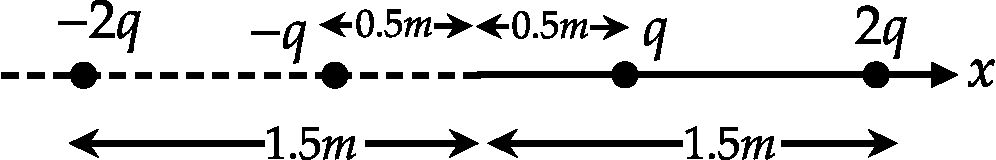
\includegraphics[height=1.2cm,width=9cm]{diagram-20210817(16)-crop}
\end{figure}
\begin{align*}
F&=\frac{q}{4 \pi \varepsilon_{0}}\left[\frac{2 q}{(1)^{2}}+\frac{q}{(1)^{2}}+\frac{2 q}{(2)^{2}}\right]\\&=\frac{q}{4 \pi \varepsilon_{0}} \times \frac{7 q}{2}\\&=\frac{1}{4 \pi \varepsilon_{0}} \frac{7 q^{2}}{2}
\end{align*}
So the correct answer is \textbf{Option (A)}
\end{answer}
\item A spherical conductor of radius $a$ is placed in a uniform electric field $\vec{E}=E_{0} \hat{k}$. The potential at a point $P(r, \theta)$ for $r>a$, is given by
$$
\Phi(r, \theta)=\text { constant }-E_{0} r \cos \theta+\frac{E_{0} a^{3}}{r^{2}} \cos \theta
$$
where $r$ is the distance of $P$ from the centre $\mathrm{O}$ of the sphere and $\theta$ is the angle OP makes with the $z$ -axis The charge density on the sphere at $\theta=30^{\circ}$ is
{\exyear{GATE 2011}}

\begin{figure}[H]
\centering
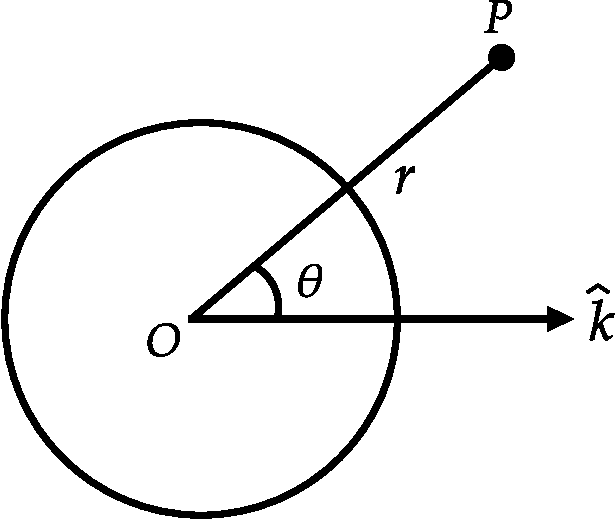
\includegraphics[height=4.2cm,width=5cm]{diagram-20210817(17)-crop}
\end{figure}
\begin{tasks}(4)
\task[\textbf{A.}] $3 \sqrt{3} \varepsilon_{0} E_{0} / 2$
\task[\textbf{B.}] $3 \varepsilon_{0} E_{0} / 2$
\task[\textbf{C.}] $\sqrt{3} \varepsilon_{0} E_{0} / 2$
\task[\textbf{D.}] $\varepsilon_{0} E_{0} / 2$
\end{tasks}
\begin{answer}
\begin{align*}
\sigma&=-\left.\varepsilon_{0} \frac{\partial V}{\partial r}\right|_{r=a}\\&=-\varepsilon_{0}\left[-E_{0} \cos \theta-\frac{2 E_{0} a^{3}}{r^{3}} \cos \theta\right]_{r=a}\\
\sigma&=-\varepsilon_{0}\left[-E_{0} \cos \theta-2 E_{0} \cos \theta\right] \Rightarrow \sigma\\&=+3 E_{0} \varepsilon_{0} \cos \theta=+3 E_{0} \varepsilon_{0} \cos 30^{\circ}\\&=\frac{3 \sqrt{3}}{2} \varepsilon_{0} E_{0}
\end{align*}
So the correct answer is \textbf{Option (A)}
\end{answer}
\item For a scalar function $\varphi$ satisfying the Laplace equation, $\vec{\nabla} \varphi$ has
{\exyear{GATE 2013}}

\begin{tasks}(2)
\task[\textbf{A.}] Zero curl and non-zero divergence
\task[\textbf{B.}] Non-zero curl and zero divergence
\task[\textbf{C.}] Zero curl and zero divergence
\task[\textbf{D.}]  Non-zero curl and non-zero divergence
\end{tasks}
\begin{answer}
\begin{align*}
\nabla^{2} \varphi&=0 \Rightarrow \vec{\nabla} \cdot(\vec{\nabla} \varphi)\\&=0\text{ and } \Rightarrow \vec{\nabla} \times(\vec{\nabla} \varphi)=0
\end{align*}
So the correct answer is \textbf{Option (C)}
\end{answer}
\item A charge distribution has the charge density given by $\rho=Q\left\{\delta\left(x-x_{0}\right)-\delta\left(x+x_{0}\right)\right\}$. For
this charge distribution the electric field at $\left(2 x_{0}, 0,0\right)$
{\exyear{GATE 2013}}

\begin{tasks}(4)
\task[\textbf{A.}] $\frac{2 Q \hat{x}}{9 \pi \varepsilon_{0} x_{0}^{2}}$
\task[\textbf{B.}] $\frac{Q \hat{x}}{4 \pi \varepsilon_{0} x_{0}^{3}}$
\task[\textbf{C.}] $\frac{Q \hat{x}}{4 \pi \varepsilon_{0} x_{0}^{2}}$
\task[\textbf{D.}] $\frac{Q \hat{x}}{16 \pi \varepsilon_{0} x_{0}^{2}}$
\end{tasks}
\begin{answer}
\begin{align*}
\text{	Potential }V(r)&=\frac{1}{4 \pi \varepsilon_{0}}\left[\int_{-a}^{a} \frac{\rho\left(x^{\prime}\right)}{x} d x^{\prime}+\int_{-a}^{a} \frac{\rho\left(x^{\prime}\right)}{x^{2}} x^{\prime} d x^{\prime}+\int_{-a}^{a} \frac{\rho\left(x^{\prime}\right)}{x^{3}} x^{\prime 2} d x^{\prime}+\ldots .\right]
\intertext{First term, total charge}
Q_{T}&=\int \rho\left(x^{\prime}\right) d x^{\prime}=Q \int_{-x_{0}}^{x_{0}} \delta\left(x^{\prime}-x_{0}\right) d x^{\prime}-Q \int_{-x_{0}}^{x_{0}} \delta\left(x^{\prime}+x_{0}\right) d x^{\prime}\\&=Q-Q=0
\intertext{Second term, dipole moment}
p&=\int x^{\prime} \rho\left(x^{\prime}\right) d x^{\prime}=Q \int_{-x_{0}}^{x_{0}} x^{\prime} \delta\left(x^{\prime}-x_{0}\right) d x^{\prime}-Q \int_{-x_{0}}^{x_{0}} x^{\prime} \delta\left(x^{\prime}+x_{0}\right) d x^{\prime}\\&=Q x_{0}-Q \times-x_{0}=2 Q x_{0}\\
V&=\frac{2 Q x_{0}}{4 \pi \varepsilon_{0} x^{2}} \Rightarrow \vec{E}=-\frac{\partial V}{\partial x} \hat{x}\\&=\frac{4 Q x_{0}}{4 \pi \varepsilon_{0} x^{3}} \hat{x}=\frac{4 Q x_{0}}{4 \pi \varepsilon_{0}\left(2 x_{0}\right)^{3}} \hat{x}\\&=\frac{Q}{8 \pi \varepsilon_{0} x_{0}^{2}} \hat{x}
\end{align*}
\end{answer}
\item A charge $-q$ is distributed uniformly over a sphere, with a positive charge $q$ at its center in (i). Also in (ii), a charge $-q$ is distributed uniformly over an ellipsoid with a positive charge $q$ at its center. With respect to the origin of the coordinate system, which one of the following statements is correct?
{\exyear{GATE 2015}}

\begin{figure}[H]
\centering
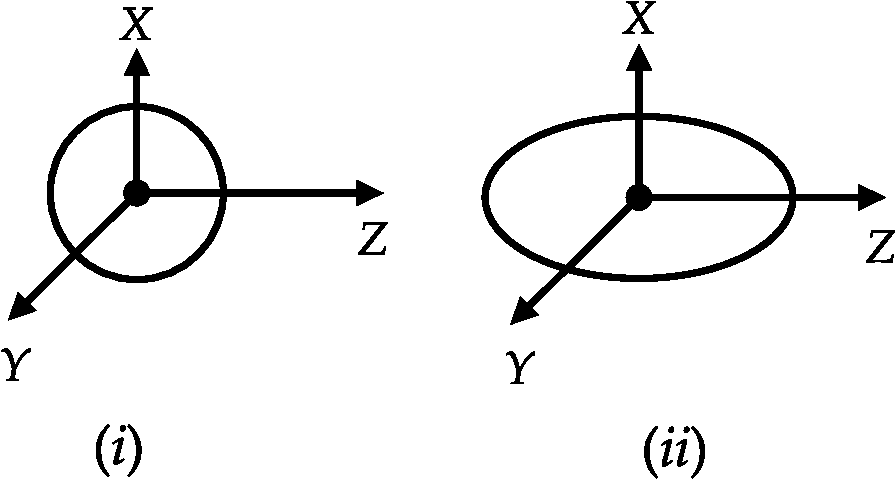
\includegraphics[height=5cm,width=10cm]{diagram-20210818(7)-crop}
\end{figure}
\begin{tasks}(1)
\task[\textbf{A.}] The dipole moment is zero in both (i) and (ii)
\task[\textbf{B.}] The dipole moment is non-zero in (i) but zero in (ii)
\task[\textbf{C.}] The dipole moment is zero in (i) but non-zero in (ii)
\task[\textbf{D.}] The dipole moment is non-zero in both (i) and (ii)
\end{tasks}
\begin{answer}
\begin{align*}
\vec{p}=\sum q_{i} \vec{r}_{i}=0\text{ in both cases.}
\end{align*}
So the correct answer is \textbf{Option (A)}
\end{answer}
\item Identical charges $q$ are placed at five vertices of a regular hexagon of side $a$. The magnitude of the electric field and the electrostatic potential at the centre of the hexagon are respectively
{\exyear{GATE 2017}}

\begin{tasks}(4)
\task[\textbf{A.}] 0,0
\task[\textbf{B.}] $\frac{q}{4 \pi \varepsilon_{0} a^{2}}, \frac{q}{4 \pi \varepsilon_{0} a}$
\task[\textbf{C.}] $\frac{q}{4 \pi \varepsilon_{0} a^{2}}, \frac{5 q}{4 \pi \varepsilon_{0} a}$
\task[\textbf{D.}]  $\frac{\sqrt{5} q}{4 \pi \varepsilon_{0} a^{2}}, \frac{\sqrt{5} q}{4 \pi \varepsilon_{0} a}$
\end{tasks}
\begin{answer}
\begin{figure}[H]
	\centering
	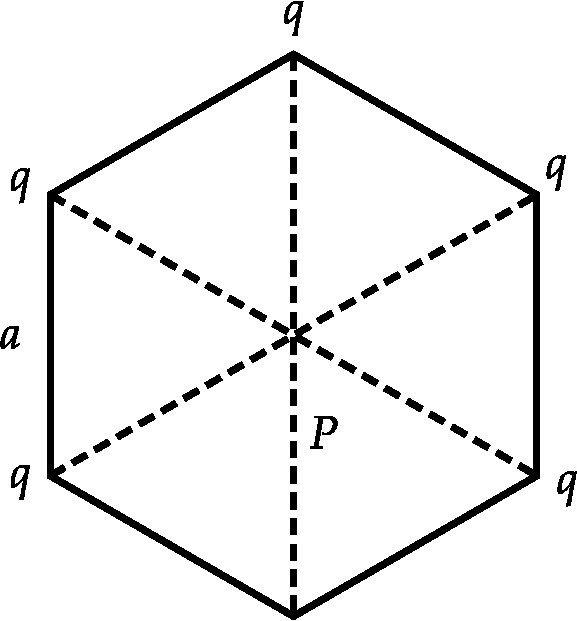
\includegraphics[height=4.3cm,width=4cm]{diagram-20210818(10)-crop}
\end{figure}
\begin{align*}
\text{The resultant field at }\mathrm{P}\text{ is }E&=\frac{q}{4 \pi \varepsilon_{0} a^{2}}\\
\text{The electrostatic potential at }\mathrm{P}\text{ is }V&=\frac{5 q}{4 \pi \varepsilon_{0} a}
\end{align*}
So the correct answer is \textbf{Option (C)}
\end{answer}
\item Three charges $(2 C,-1 C,-1 C)$ are placed at the vertices of an equilateral triangle of side $1 m$ as shown in the figure. The component of the electric dipole moment about the marked origin along the $\hat{y}$ direction is-------$C m$.
{\exyear{GATE 2017}}

\begin{figure}[H]
\centering
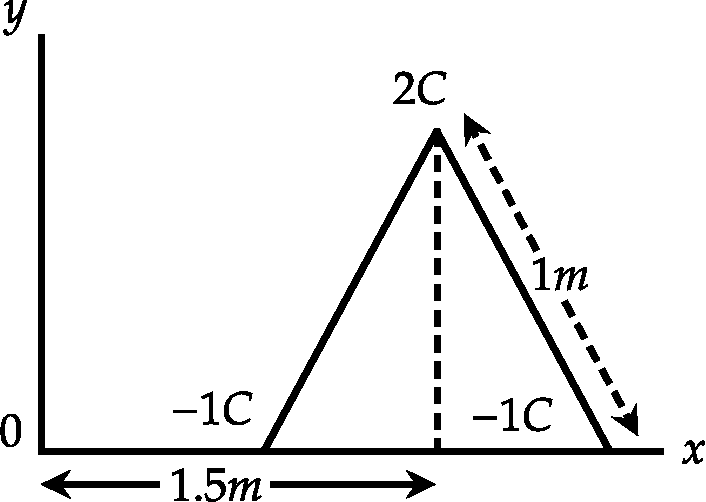
\includegraphics[height=4.5cm,width=6cm]{diagram-20210818(11)-crop}
\end{figure}
\begin{answer}
\begin{align*}
\vec{p}&=-1(1 \hat{x})-1(2 \hat{x})+2(1.5 \hat{x}+\sqrt{1-0.25} \hat{y})\\
\text{	Along the }\hat{y}\text{ direction }&=2 \times \sqrt{1-0.25}=1.73
\end{align*}
\end{answer}
	\item Consider a system of three charges as shown in the figure below:\\
\begin{figure}[H]
	\centering
	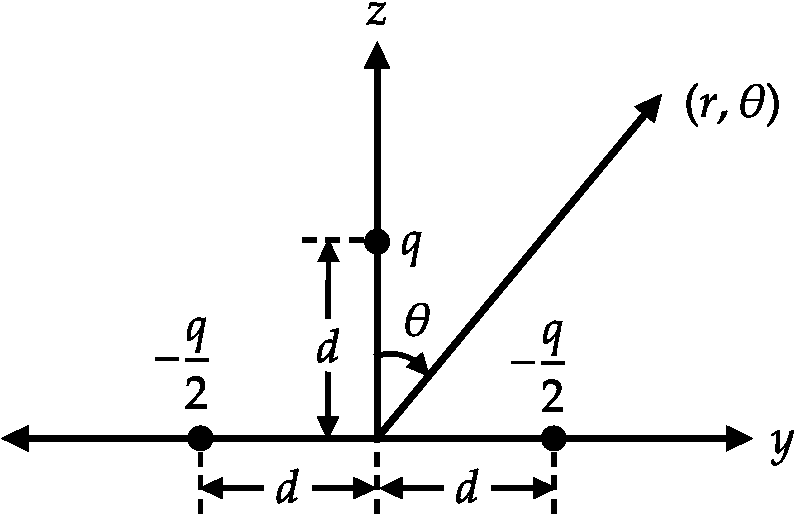
\includegraphics[height=4.5cm,width=7cm]{diagram-20210818(17)-crop}
\end{figure}
 For $r=10 \mathrm{~m} ; \theta=60$ degrees; $q=10^{-6}$ Coulomb, and $d=10^{-3} \mathrm{~m}$, the electric dipole potential in volts (rounded off to three decimal places) at a point $(r, \theta)$ is--------- [Use: $\left.\frac{1}{4 \pi \in_{0}}=9 \times 10^{9} \frac{\mathrm{Nm}^{2}}{C^{2}}\right]$
{\exyear{GATE 2019}}

\begin{answer}
\begin{align*}
\text{Monopole moment }&=-\frac{q}{2}-\frac{q}{2}+q=0\\
\vec{p}&=-\frac{q}{2} \times(-d \hat{y})-\frac{q}{2}(d \hat{y})+q(d \hat{z})\\
\vec{p}&=q d \hat{z}\\
V(r, \theta)&=\frac{1}{4 \pi \in_{0}} \frac{\vec{p} \cdot r}{r^{2}}=\frac{1}{4 \pi \in_{0}} \frac{q d \cos \theta}{r^{2}}\\
V(r, \theta)&=9 \times 10^{9} \times \frac{10^{-6} \times 10^{-3} \times \cos 60^{\circ}}{(10)^{2}}\\
&=9 \times 10^{9} \times \frac{10^{-9}}{2 \times 100}=0.045
\end{align*}
\end{answer}
\end{enumerate}
\colorlet{ocre1}{ocre!70!}
\colorlet{ocrel}{ocre!30!}
\setlength\arrayrulewidth{1pt}
\begin{table}[H]
	\centering
	\arrayrulecolor{ocre}
	\begin{tabular}{|p{1.5cm}|p{1.5cm}||p{1.5cm}|p{1.5cm}|}
		\hline
		\multicolumn{4}{|c|}{\textbf{Answer key}}\\\hline\hline
		\rowcolor{ocrel}Q.No.&Answer&Q.No.&Answer\\\hline
		1&\textbf{C} &2&\textbf{A}\\\hline 
		3&\textbf{A} &4&\textbf{C} \\\hline
		5&\textbf{A} &6&\textbf{A} \\\hline
		7&\textbf{C}&8&\textbf{1.73}\\\hline
		9&\textbf{0.045}&10&\textbf{}\\\hline
		11&\textbf{} &12&\textbf{}\\\hline
		13&\textbf{}&14&\textbf{}\\\hline
		15&\textbf{}& &\\\hline
		
	\end{tabular}
\end{table}